\section{Method of Regularized Stokeslets}
\subsection{Stokes flow}
When we look at many physical systems, particularly in biology, we find that the inertial forces withing the fluid are small in comparison to that of the viscous terms. In these cases we can take the limit of the Navier-Stokes equation (\cref{eq:NavierStokes})where $R e=\rho u L/\mu \to 0 $ \cite{Trombley2019BasicFlows}. Within biological system we find that these cases occur when either we are looking at highly viscous fluids where $\mu$ is large or at small length scales where $L$ (The typical scale of the system) is very small such as when looking looking at cells, microorganism or flows around small capillaries \cite{Blake1972AOrganisms, Higdon1979APropulsion, Smith2009MathematicalFluids}. As well as biological models we can use it in more general fluid dynamics, where we have stokes flow, with complex boundaries \cite{Liron1978StokesPipe, Liron1976StokesPlates}. 

The steady state Stokes equations in two or three dimensions are
\begin{subequations}
\label{eq:StokesFlow}
\begin{align}
    \mu\Delta\boldsymbol{u} &= \nabla p - \boldsymbol{F} \label{eq:StokesFlow1} \\ 
    \nabla \cdot \boldsymbol{u} &= 0 \label{eq:StokesFlow2}
\end{align}
\end{subequations}
where $\mathbf{u}$ is the velocity of the fluid, $\mathbf{F}$ is the external force, $p$ is the pressure and $\mu$ is the fluid viscosity.
We can derive a singular fundamental solution to the Stokes equations which we will call a \textit{Stokeslet}. The Stokeslet represents the solution for the velocity of the fluid given that the external force $\mathbf{F}$ acting on the fluid is concentrated at a single point $\mathbf{F} = \mathbf{f_0}\delta(\mathbf{x})$ \cite{Hancock1953TheLiquids, Batchelor2000AnDynamics, Pozrikidis1992BoundaryFlow}.
Through Similar methods to that show later for deriving regularised Stokeslet Equation (\cref{eq:regstokeslet2}) we can derive the singular fundamental solutions to the stokes equations as 
\begin{equation*}
\begin{aligned}
    S_{j k}(\mathbf{x}, \mathbf{x_0}) &= \frac{\delta_{j k}}{r}+\frac{\left(x_{j}-x_{0,j}\right)\left(x_{k}-x_{0,k}\right)}{r^{3}} \\
    P_{k}(\mathbf{x}, \mathbf{x_0}) &= \frac{x_{k}-x_{0,k}}{r^{3}} \\
    T_{ijk}(\mathbf{x}, \mathbf{x_0}) &= \frac{-6\left(x_{i}-x_{0,i}\right)\left(x_{j}-x_{0,j}\right)\left(x_{k}-x_{0,k}\right)}{r^5}
\end{aligned}
\end{equation*}
Where $r=|\mathbf{x}-\mathbf{x_0}|$. We find the velocity $\mathbf{u}$ at a point $\mathbf{x}$ through the equation  
\begin{equation*}
    \mathbf{u} = (8 \pi \mu)^{-1} \left(S_{1k},S_{2k},S_{3k}\right)f_{0,j}
\end{equation*} 
where $\mathbf{f_{0}}$ is the force per unit area, exerted by the fluid on the surface, concentrated at the point $\mathbf{x_0}$.


\subsection{Regularising the Stokeslet}
While the singular Stokeslet provides a useful mechanism to solve boundary integral equations, it relies on the surfaces on which they are concentrated on to be smooth such that the velocity is integrable and the fluid bounded in the neighbourhood of the surface. However if we consider non smooth surfaces or curves instead of surfaces then the resulting equations for velocity become non singular and much harder so work with. 

\begin{figure}
    \centering
    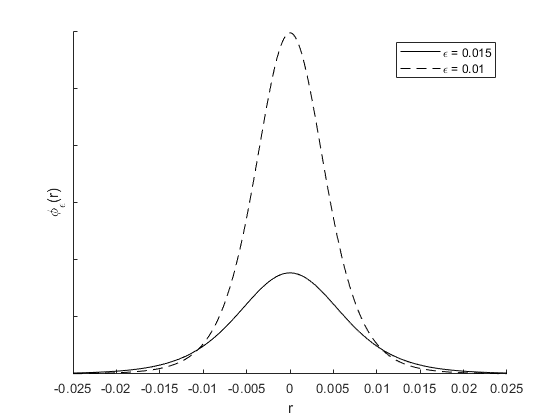
\includegraphics[scale=0.65]{Images/BlobFunction.png}
    \caption{Blob function in equation \cref{eq:blobfunc} for several values of epsilon}
    \label{fig:blobfunc}
\end{figure}

In order to remove these singularities we use a "blob function" which instead of approximating at force at a singular point we instead approximate as a sphere centred at the the same point. While the radius of the sphere is often infinite the blob function decays rapidly away from the centre with the largest contribution obtained in the close vicinity of the centre. We introduce a control parameter $\epsilon$ independent of any discretization which controls the rate of decay. The effect of this control parameter can be seen in Fig.\ref{fig:blobfunc}. In order to obtain similar results to that of the singular solutions we dictate that $\int \phi_\epsilon(r)dr=1$ for all values of $\epsilon$. This allows us to preserve the results obtained for the singular kernels for distances away from the point in which the force is exerted and obtains different results close to the point. In order to retain the singular solution we have that as $\epsilon \to 0$ our blob function must tend to the Dirac delta. For simplicity of the paper and the application to wider range of problems we will only consider spherically symmetric function such as those in \cref{eq:blobfunc,eq:blobfunc2} \cite{Cortez2005,Olson2013ModelingFormulation,Nguyen2014ReductionFlow}.
\begin{equation}
\label{eq:blobfunc}
    \phi_\epsilon(r)= \frac{15 \epsilon^4}{8\pi\left( r^2 +\epsilon^2 \right)^{7/2}}
\end{equation}

\begin{equation}
\label{eq:blobfunc2}
    \psi_{\epsilon}(r)=\frac{15 \epsilon^{6}\left(5-\frac{2 r^{2}}{\epsilon^{2}}\right)}{16 \pi\left(r^{2}+\epsilon^{2}\right)^{9 / 2}} \quad\quad \phi_{\epsilon}(r)=\frac{5 \epsilon^{2}-2 r^{2}}{2 \pi^{3 / 2} \epsilon^{5}} e^{-r^{2} / \epsilon^{2}}
\end{equation}
For the derivation of the regularised Stokeslets and all further numerical analysis we will use \cref{eq:blobfunc} due to its popularity in external literature and the simplicity of the kernel it generates.

\subsubsection{Derivation of the Stokeslet}
By concentrating the force onto a singular point using the blob function we convert the stokes equations given in \cref{eq:StokesFlow} to a new set of equation for which we will derive the solution,
\begin{subequations}
\label{eq:RegStokesFlow}
\begin{align}
    \mu\Delta\boldsymbol{u} &= \nabla p - \phi_{\epsilon}(\mathbf{x}-\mathbf{x_0})\mathbf{f_0} \label{eq:RegStokesFlow1} \\ 
    \nabla \cdot \boldsymbol{u} &= 0 \label{eq:RegStokesFlow2}
\end{align}
\end{subequations}
where $f_0$ is the force per unit area as define in the previous section.
In order to simplify notation from this point on-wards we will use the Einstein summation convention where repeated indices are summed over. We introduce the regularised Stokeslet function $S^\epsilon(\mathbf{x},\mathbf{x_0})$ which is the Green's function for the velocity. We can now write the solution to \cref{eq:RegStokesFlow} as 
\begin{equation}
\label{eq:regvelsol}
    u_i(\mathbf{x}) = \frac{1}{8\pi\mu}S^\epsilon_{ij}(\mathbf{x},\mathbf{x_0})f_{0,j}
\end{equation}
The pressure and stress tensor associated with that flow can also be also be written as
\begin{equation}
\label{eq:regpressuresol}
    p(\mathbf{x}) = \frac{1}{8\pi}P^\epsilon_{j}(\mathbf{x},\mathbf{x_0})f_{0,j}
\end{equation}
\begin{equation}
\label{eq:regstresssol}
    \sigma_i(\mathbf{x}) = \frac{1}{8\pi}T^\epsilon_{ijk}(\mathbf{x},\mathbf{x_0})f_{0,j}
\end{equation}
By substituting these solutions back into \cref{eq:RegStokesFlow1} we find that they must obey
\begin{equation}
\label{eq:regcondition1}
    \Delta S^\epsilon_{kj}(\mathbf{x},\mathbf{x_0}) = \frac{\partial P^\epsilon_{j}(\mathbf{x},\mathbf{x_0})}{\partial x_k} - 8\pi\delta_{kj}\phi_\epsilon(\mathbf{x}-\mathbf{x_0})
\end{equation}
for all j and k with $\delta_{kj}$ being the Kronecker delta. The impressibility condition \cref{eq:RegStokesFlow2} also gives us that
\begin{equation}
\label{eq:regcondition2}
    \frac{\partial S^\epsilon_{ij}(\mathbf{x},\mathbf{x_0})}{\partial x_i} = 0
\end{equation}
for all j. We next take the derivative of \cref{eq:regcondition1} with respect to $x_k$ to get 
\begin{equation*}
    \frac{\partial S^\epsilon_{kj}(\mathbf{x},\mathbf{x_0})}{\partial x_i \partial x_i \partial x_k} = \frac{\partial^2 P^\epsilon_{j}(\mathbf{x},\mathbf{x_0})}{\partial x_k^2} - 8\pi\delta_{kj}\frac{\partial \phi_\epsilon(\mathbf{x}-\mathbf{x_0})}{\partial x_k}
\end{equation*}
Summing over $k$ as per the convention and using \cref{eq:regcondition2} gives us 
\begin{equation}
\label{eq:regpressureeq}
    \Delta P^\epsilon_{j}(\mathbf{x},\mathbf{x_0}) = 8\pi\frac{\partial \phi_\epsilon(\mathbf{x}-\mathbf{x_0})}{\partial x_j}
\end{equation}
If we now introduce the following two equations for simplicity
\begin{subequations}
\label{eq:intermediate}
\begin{align}
    \Delta G^\epsilon(\mathbf{x}-\mathbf{x_0})  &= \phi_\epsilon(\mathbf{x}-\mathbf{x_0}) \label{eq:inter1} \\
    \Delta B^\epsilon(\mathbf{x}-\mathbf{x_0})  &= G^\epsilon(\mathbf{x}-\mathbf{x_0}) \label{eq:inter2}
\end{align}
\end{subequations}
Using \cref{eq:inter1,eq:regpressureeq} we can express the pressure as 
\begin{equation}
\label{eq:pressuresol}
    P^\epsilon_{j}(\mathbf{x},\mathbf{x_0})f_{0,j} = 8 \pi \frac{\partial G^\epsilon(\mathbf{x}-\mathbf{x_0})}{\partial x_j}
\end{equation}
Then finally using \cref{eq:regcondition2,eq:inter2} gives us the general for of our Stokeslet.
\begin{equation}
\label{eq:regstokeslet1}
    s_{ij}^\epsilon(\mathbf{x}, \mathbf{x_0}) = 8\pi\left[ \frac{\partial^2 B^\epsilon(\mathbf{x} -\mathbf{x_0})}{\partial x_i \partial x_j} - \delta_{ij}  G^\epsilon(\mathbf{x} -\mathbf{x_0})\right]
\end{equation}
As the stress tensor is defined as 
\begin{equation*}
    \sigma_{ij}(\mathbf{x}) = -\delta_{ik}p(\mathbf{x}) + \mu\left( \frac{\partial u_i}{\partial x_k} + \frac{\partial u_k}{\partial x_i} \right)
\end{equation*}
we find that 
\begin{equation}
\label{eq:regDoubleLayerSol}
    T^\epsilon_{ijk}(\mathbf{x},\mathbf{x_0}) = -\delta_{ik} P^\epsilon_j(\mathbf{x},\mathbf{x_0}) + \mu\left( \frac{\partial S^\epsilon_{ij}(\mathbf{x},\mathbf{x_0})}{\partial x_k} + \frac{\partial S^\epsilon_{kj}(\mathbf{x},\mathbf{x_0})}{\partial x_i}\right)
\end{equation}

\subsubsection{Specific Blob}
If we take the blob equation defined in \cref{eq:blobfunc} and solve to find $G^\varepsilon$ and $B^\varepsilon$ we get that
\begin{subequations}
\begin{align}
    G^\varepsilon(\mathbf{x}-\mathbf{x_0}) &= \frac{-2r^2+3\epsilon^2}{8\pi(r^2+\epsilon^2)^{3/2}} + \frac{3}{8\pi\epsilon} \label{eq:G}\\
    B^\varepsilon(\mathbf{x}-\mathbf{x_0}) &= -\frac{\sqrt{\epsilon^2+r^2}}{8\pi} + \frac{r^2}{16\pi\epsilon} + \frac{\epsilon}{8\pi}\label{eq:B}\\\
\end{align}
\end{subequations}
where $r=|\mathbf{x}-\mathbf{x_0}|$. We now substitute \cref{eq:G,eq:B} into \cref{eq:pressuresol,eq:regstokeslet1,eq:regDoubleLayerSol} to obtain our final kernels which will be used for all further analysis.

\begin{subequations}
\begin{align}
    P_j^\epsilon(\mathbf{x}, \mathbf{x_0}) =& (x_j-x_{0,j})\frac{2r^2+5\epsilon^2}{(r^2+\epsilon^2)^{5/2}} \label{eq:pressuresol2}\\
    S_{ij}^\epsilon(\mathbf{x}, \mathbf{x_0}) =& \delta_{ij} \frac{r^2+2\epsilon^2}{\left( r^2 + \epsilon^2 \right)^{3/2}} + \frac{(x_i-x_{0i})(x_j-x_{0j})}{\left( r^2 + \epsilon^2 \right)^{3/2}} \label{eq:regstokeslet2} \\ 
    T_{ijk}^\epsilon(\mathbf{x}, \mathbf{x_0}) =& \frac{-6(x_i-x_{0,i})(x_j-x_{0,j})(x_k-x_{0,k})}{(r^2+\epsilon^2)^{5/2}} \label{eq:doublelayer2}\\
    &-\frac{3\epsilon^2[\delta_{jk}(x_i-x_{0,i}) +\delta_{ik}(x_j-x_{0,j})+\delta_{ij}(x_k-x_{0,k})]}{(r^2+\epsilon^2)^{5/2}} \nonumber
\end{align}
\end{subequations}
We can easily check that these provide results consistent with those found by the singular solutions as in the limit $\epsilon \to 0$ we obtain the same results stated in the previous section.


\begin{equation}
    \int_{\mathbb{R}^{3}} u_{j}(\mathbf{x}) \phi_{\epsilon}\left(\mathbf{x}-\mathbf{x}_{0}\right) d V(\mathbf{x})=-\frac{1}{8 \pi \mu} \int_{\partial D} S_{i j}^{\epsilon}\left(\mathbf{x}, \mathbf{x}_{0}\right) f_{i} d s(\mathbf{x})
\end{equation}


\begin{equation}
\label{eq:Stokesletsum}
    u_{j}\left(\mathbf{x}_{0}\right)=\frac{1}{8 \pi \mu} \sum_{n=1}^{N} \sum_{i=1}^{3} S_{i j}^{\epsilon}\left(\mathbf{x}_{n}, \mathbf{x}_{0}\right) f_{n, i} A_{n}
\end{equation}